\section*{\centering R\'esum\'e}

Dans cette th\`ese, nous \'etudions le probl\`eme d'optimisation s\'equentielle dans des enviro\-nnements stochastiques. A chaque instant, nous pouvons interroger un point de l'enviro\-nnement, et recevoir une récompense bruit\'ee. Nous nous concentrons d'abord sur le cas o\`u l'environnement est représenté par un nombre fini de points, et ensuite sur le cas plus g\'en\'eral o\`u l'environnement est composé d'un nombre infini d\'enombrable de points, voire continu. Dans les deux cas, le co\^ut d'une requ\^ete pouvant \^etre \'elev\'ee, nous envisageons ainsi \`a rep\'erer au plus vite le point (quasi)-optimal. Cette \'etude est motiv\'ee par de nombreux sc\'enarios r\'eels comme, entre autres, les essais cliniques, les tests A/B, ou l'optimisation des placements publicitaires. Ainsi pour terminer, nous nous int\'eressons en particulier \`a l'une de ces applications plus importantes pour la communaut\'e d'apprentissage statistique, c'est-\`a-dire l'optimisation des hyper-param\`etres.

\begin{center}
    \rule{8cm}{0.4pt}
\end{center}

\section*{\centering Abstract}

In this thesis, we study the problem of sequential optimization under stochastic environments. At each round, we can query a data point from the environment, and receive a noisy reward. We first focus on the case where the environment is abstracted as a finite search space, then we investigate also on a more general setting where the environment is composed of an infinite number of points or even continuous. In both cases, the cost of a single query would be high, and we thus aim at identify the (near)-optimum as efficiently as possible. The whole study is motivated by numerous real scenarios including, but not limited to, clinical trial, A/B testing, advertisement placement optimization. We therefore conclude by some particular focus on one of its most important contributions for the machine learning community, \emph{i.e.} hyper-parameter optimization.


\chapter*{R\'esum\'e des travaux de thèse}
    %\addcontentsline{toc}{chapter}{R\'esum\'e des travaux de thèse (in French)}

\section{Contexte de la th\`ese}\label{sec:abs.context}
	
\subsection{Qu-\'etudions-nous et pourquoi ?}\label{sec:abs.context.what}

Imaginons que nous ayons accès à un simulateur qui modélise le comportement d'une tâche numérique complexe. Considéré comme une boîte noire, nous ne pouvons obtenir des informations utiles qu'en exécutant le simulateur avec différentes entrées. Par exemple, le processus d'inférence de la structure 3D d'une protéine à partir de sa séquence d'acides aminés peut être considéré comme une tâche complexe, qui peut être modélisée par un simulateur. Les entrées du simulateur sont les séquences d'acides aminés et les sorties sont les structures 3D prédites. Une famille populaire de méthodes cherche à optimiser une fonction énergétique appropriée - produite par le simulateur - qui décrit la relation entre la structure d'une protéine et sa séquence d'acides aminés. Ces méthodes sont intéressantes car elles sont capables de construire des structures de protéines sans connaissance préalable des structures résolues (voir par exemple ~\citealt{zhang2008}).

Dans le contexte de cette thèse, nous modélisons un tel scénario comme le problème dit de l'optimisation séquentielle, dans lequel un agent alimente séquentiellement un environnement (le simulateur dans l'exemple précédent) avec des entrées et reçoit un retour (déterministe ou stochastique) appelé gain, récompense ou observation. L'agent doit produire une estimation de l'entrée optimale après un certain nombre d'essais. Dans certaines circonstances, une seule interaction avec l'environnement peut être extrêmement coûteuse. Par exemple, dans l'exemple de la prédiction de la structure des protéines, de vastes ressources informatiques sont nécessaires si le simulateur reçoit une très grande protéine (avec de longues séquences d'acides aminés). Il est donc très intéressant de choisir soigneusement l'entrée à chaque pas de temps en fonction des observations passées afin de réduire le nombre de simulations.

L'optimisation séquentielle dans des environnements stochastiques est un sujet de recherche actif dans les communautés des mathématiques appliquées et de l'informatique. Par exemple, le problème de planification dans un processus de d\'ecision markovien, sur lequel la récente percée de l'intelligence de jeu du Go~\citep{silver2016alphago} est construite, est étroitement lié à l'optimisation séquentielle. Précisément, étant donné l'état actuel du jeu, l'intelligence de jeu est conçue pour maximiser une certaine fonction de valeur, dont les observations (bruitées) peuvent être obtenues en explorant des trajectoires bien choisies.

Un autre exemple, qui est aussi une motivation importante pour cette thèse, est celui de l'optimisation des hyper-paramètres des classifieurs d'apprentissage automatique. Les algorithmes modernes d'apprentissage automatique dépendent souvent de nombreux paramètres qui ne peuvent pas être appris par le processus d'apprentissage, mais qui doivent être spécifiés manuellement. Le réglage de ces hyper-paramètres est souvent considéré comme une partie fastidieuse d'une tâche d'apprentissage automatique. Il est donc intéressant de concevoir des algorithmes qui automatisent le processus de choix de ces hyper-paramètres. L'optimisation des hyper-paramètres peut être considéré comme un problème d'optimisation bo\^itre noire où les évaluations de fonctions sont supposées être très coûteuses. En général, l'évaluation d'une fonction dans l'optimisation des hyper-paramètres implique l'exécution complète de l'algorithme principal d'apprentissage automatique sur un ensemble de données important et hautement dimensionnel, ce qui prend souvent beaucoup de temps ou de ressources.

En outre, l'optimisation séquentielle peut également servir d'abstraction pour de nombreux problèmes du monde réel. Pour n'en citer que quelques-uns, on peut penser aux problèmes de sélection de portefeuille (averse au risque) en finance~\citep{ziemba2010}, à la conception de stratégies efficaces d'allocation de traitement en médecine~\citep{durand2018contextual}, à la minimisation de l'énergie libre en génie chimique ou à la prédiction de la structure des protéines~\citep{floudas2000}, à la métamodélisation pour l'optimisation de la conception technique~\citep{wang2007}, à la estimation des paramètres (problème inverse) des voies biochimiques dynamiques non linéaires~\citep{moles2003}, à la distorsion du maillage en science des matériaux~\citep{charpagne2019ebsd}, et bien plus encore. 

Pour résumer, un environnement peut simplement être considéré comme une fonction cible à optimiser. Cette fonction peut être \textbf{discrète ou continue}. Dans cette thèse, nous nous intéressons en particulier à l'optimisation de fonctions pour lesquelles \textbf{aucune (ou peu)} hypothèse de régularité est faite, et seules des évaluations de fonctions (interactions avec l'environnement) \textbf{bruitées     (ou stochastiques)} peuvent être observées.

%Le problème de planification dans un Processus de Décision Markovien (MDP pour Markov Decision Process, [1]), pouvant modéliser la gestion de ressources dans un système de type smart grids ou encore le contrôle d'un robot, et celui de la construction d'intelligences artificielles pour des jeux, sont très liés à celui de l'optimisation séquentielle puisqu'ils reviennent à déterminer l'action qui dans un état donné maximise une fonction valeur, dont on peut obtenir des réalisations bruitées en explorant des trajectoires bien choisies.

%In this context, since one does not make extra regularity assumptions on the target function, one can imagine that it can be very costly to evaluate the function. Thus a good strategy for choosing adaptively the next observation is needed in order to find an optimal (or quasi-optimal) point with as few number of evaluations as possible. This is the sequential optimization problem. That being said, the main problematic of my thesis is the \emph{global sequential optimization} problem. Several applications could be investigated in this thesis, in particular the \emph{automatic hyper-parameter tuning} of machine learning algorithms~\citep{samothrakis2013,hoffman2014bayesgap,jamieson2016hyperband,li2017hyperband}.

\subsection{Comment traitons-nous le probl\`eme ?}\label{sec:abs.context.how}

L'outil principal que nous utilisons pour traiter le problème d'optimisation séquentielle dans cette thèse est un modèle statistique qui s'appelle le modèle de bandit à plusieurs bras. Ce modèle a été étudié pour la première fois par~\cite{thompson1933}, et peut être décrit de la manière suivante : On donne à un agent un ensemble \emph{fini} de bras $K$ et un horizon $N$. Tirer un bras conduit à une récompense stochastique qui suit une certaine distribution \emph{inconnue} sous ce bras. À chaque pas de temps, l'agent peut choisir de tirer l'un des bras et observe une récompense échantillonnée à partir de sa distribution sous-jacente correspondante.

% \begin{remark}\label{remark:partial}
% \begin{leftbar}[remarkbar]
% Note that rewards of unchosen arms at each time step are not revealed: this partially observable feedback setting is thus a special case of the online learning with experts setting.
% \end{leftbar}
% \end{remark}

Dans son article de référence,~\cite{robbins1952} définit l'objectif d'un agent de bandits comme la maximisation des récompenses totales à long terme. On observe que l'agent doit simultanément acquérir de nouvelles informations en vue d'un bien-être potentiel futur (exploration), et optimiser la décision actuelle basée sur les observations passées (exploitation). Ce phénomène est le fameux \emph{dilemme de l'exploration et l'exploitation} et est présent dans de nombreuses tâches du monde réel. Le modèle de bandits est donc populaire parmi différentes communautés, car les algorithmes font un compromis entre l'exploration et l'exploitation.
%The usual performance criterion of the learner is measured by the total loss of the chosen arm at each time step w.r.t the best arm, namely the \emph{cumulative regret}. Typical good learners like \UCB~\citep{auer2002ucb} trade off between exploration and exploitation. 

Cependant, l'exploitation ne fournit pas nécessairement des incitations significatives dans certaines applications réelles. Typiquement, dans les exemples précédents présentés dans la section~\ref{sec:abs.context.what}, nous ne nous soucions pas vraiment des pertes potentielles encourues pendant toute la phase d'apprentissage. En effet, nous cherchons uniquement à trouver rapidement le (quasi-)optimum de la fonction cible. Dans ce contexte, il est plus naturel d'évaluer l'agent dans une optique d'optimisation. Ce cadre, souvent appelé \emph{identification du meilleurs bras}, est donc plus fortement lié à ce que nous allons étudier dans cette thèse. L'identification du meilleurs bras a été étudié en premier lieu par~\cite{even-dar2003confidence} et~\cite{bubeck2009pure} dans deux cadres différents que nous présentons en détail dans le chapitre~\ref{CHAP:MAB}.

Plus généralement, nous parlons de problèmes de \emph{l'exploration pure}~\citep{bubeck2011pure}, où l'agent est censé gagner autant d'informations possibles sur le modèle de bandit indépendamment des récompenses. L'identification du meilleurs bras est simplement une instance particulière de l'exploration pure, pour laquelle l'objectif d'apprentissage est de trouver le bras optimal. D'autres objectifs d'apprentissage existent également, comme trouver des bras qui dépassent un certain seuil prédéfini (voir par exemple ~\citealt{locatelli2016thresholding}). Cependant, nous nous concentrons principalement sur l'identification du meilleurs bras dans cette thèse car il a un large éventail d'applications.

\subsection{Du bandit manchot \`a l'apprentissage par renforcement}\label{sec:abs.context.rl}

Le modèle de bandits est populaire d'un autre point de vue car certains problèmes de bandits font partie d'un cadre plus général qui est l'apprentissage par renforcement (RL). Dans un modèle du RL, l'environnement est caractérisé par son état actuel et l'agent interagit avec l'environnement en prenant différentes actions. Chaque action conduit à une récompense de la part de l'environnement ainsi qu'à un changement d'état. La définition formelle et les résultats généraux du RL dépassent le cadre de cette thèse, les lecteurs peuvent se référer à~\cite{sutton1998,bertsekas2011approximate} pour les études. 

L'apprentissage par renforcement moderne combiné avec l'apprentissage profond a conduit à des avancées passionnantes, notamment AlphaGo~\citep{silver2016alphago}, AlphaStar~\citep{vinyals2019alphastar}, etc. Cependant, il existe encore une grande lacune dans la compréhension de l'énorme succès de RL profond. Bandit manchot, en tant que modèle statistique fortement fondé par la théorie, peut potentiellement servir de première étape pour combler cette lacune dans la recherche sur le RL profond. Plus précisément, bandit manchot est parfois considéré comme la forme la plus simple de RL car les agents de bandits ne subissent aucun changement d'état (voir Fig.~\ref{fig:abs.comparison}). Nous discuterons un peu plus du lien entre bandits et RL plus tard dans la conclusion générale~\ref{CHAP:CONCLUSION} car les bandits contextuelles (bandits avec informations secondaires) -- une variante du modèle classique -- décrit finalement mieux la façon dont le bandit manchot est lié au RL.

\begin{figure}[ht]
    \centering
    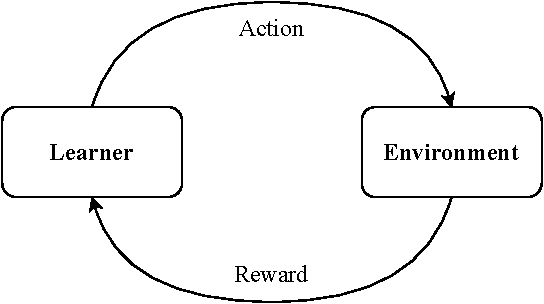
\includegraphics[width=0.33\textwidth]{Chapter0/img/mab.pdf}
    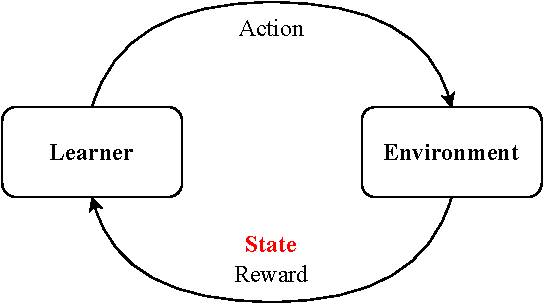
\includegraphics[width=0.33\textwidth]{Chapter0/img/rl.pdf}
    \caption{Gauche: cycle d'apprentissage bandit vs. Droite: cycle d'apprentissage RL.}
    \label{fig:abs.comparison}
\end{figure}

\section{Bandit manchot multi-bras et optimisation}\label{sec:abs.mab}
    
Cette thèse traite des problèmes d'optimisation séquentielle dans des environnements stochastiques en utilisant des outils de bandits. Un environnement stochastique se réfère à un environnement à partir duquel des retours stochastiques sont acquis lorsqu'une entrée est demandée depuis l'espace de recherche/action\footnote{Ces termes peuvent être employés de manière interchangeable.} $\mathcal{X}$. Formellement, et sans perte de généralité, notre objectif est de maximiser une fonction cible $f:\mathcal{X}\rightarrow\mathbb{R}$, c'est-à-dire de trouver 
\begin{equation}\label{eq:abs.optim}
    \argmax_{x\in\cX} f(x)
\end{equation}
en fonction d'une séquence de valeurs de la fonction $f$. Évidemment, sans aucune information préalable sur la fonction cible et/ou l'espace de recherche $\cX$, il s'agit d'une mission impossible. Cette thèse étudie plusieurs instances particulières de \eqref{eq:abs.optim} avec différents espaces de recherche et/ou différentes hypothèses (de régularité) sur la fonction cible, et apporte de nouvelles perspectives théoriques et pratiques. 

Dans le reste de ce chapitre, je donne un aperçu informel des différents contextes étudiés dans cette thèse ainsi qu'un résumé de mes contributions à chaque contexte.

Une discussion plus approfondie sur la formulation du problème, en particulier sur la manière d'évaluer la performance des algorithmes dans différents contextes, est donnée dans le chapitre~\ref{CHAP:MAB}, qui constitue une introduction au modèle de bandit. L'objectif de ce chapitre introductif est de présenter le problème de bandits de manière plus formelle. Nous rappelons d'abord quelques notions de base ainsi que certains résultats fondamentaux pour les bandits stochastiques. Nous nous concentrons ensuite sur la façon dont différents cadres d'identification du meilleur bras sont formulés.

%In its simplest form where the action space $\mathcal{X}$ is finite, the problem can be modeled as a \emph{stochastic multi-armed bandit}. The term \emph{bandit} is named, by analogy, after slot machines (or one-armed bandits) in a casino. A \emph{sequential decision making} problem comes up then when facing with several slot machines (multi-armed bandits). Concretely, a stochastic bandit is a collection of $K$ actions (also called arms) $\mathcal{X} = \{x_1,\ldots,x_K\}$. Each time the learner chooses one action $x_{a_t}\in\mathcal{X}$ which is then fed to the environment. The environment generates a reward $r_{a_t,t}=r_t$ which is assumed to be drawn from an unknown $[0,1]$-valued distribution $\nu_{a_t}$ and is revealed to the learner.

%In its original formulation, the learning objective of a stochastic bandit is to maximise the total reward $\sum_{t=1}^T r_t$ obtained within a given time horizon $T$. In the literature of bandit, we usually denote by $\mu_k$ (resp. $\mu^\star$) the expectation of the unknown distribution $\nu_k$ (resp. the optimal arm), and the previous reward maximisation objective is equivalent to minimising the \emph{cumulative regret}: $T\mu^\star-\sum_{t=1}^T \mu_{a_t}$. %A such learning objective requires the learner to simultaneously acquire new information for potential future well-being (called \emph{exploration}), and optimize the current decision based on past observations (called \emph{exploitation}). 
%Multi-armed bandits naturally addresses the trade-off between exploration and exploitation.

\subsection{Identification du meilleurs bras dans un modèle de bandit stochastique}\label{sec:abs.mab.bai}

Le premier cadre d'intérêt consiste en un espace de recherche fini et unidimensionnel $\cX = \{x_1,x_2,\cdots,x_K\}$. Supposons que la distribution de récompense sous-jacente du bras $x_k$ soit caractérisée par sa moyenne $\mu_k\in\R$, la fonction cible $f$ peut être simplement interprétée comme une correspondance entre chaque bras et sa moyenne. L'agent cherche alors à trouver
\begin{align}\label{eq:abs.optim_bai}
    \argmax_{k\in[K]} \mu_k\,
\end{align}
étant donné une certaine condition d'arrêt. Il s'agit de l'identification du meilleur bras pour les bandits multi-bras stochastiques. Il existe plusieurs objectifs d'apprentissage pour ce genre de problèmes, parmi lesquels nous sommes particulièrement intéressés par le cas où le but est d'identifier le meilleur bras avec une confiance élevée avec un minimum d'évaluations de fonctions. Il s'agit du \emph{cadre dit de confiance fixée} pour lequel la définition formelle, ainsi que celles pour d'autres objectifs d'apprentissage, sont fournies et discutées plus loin dans le chapitre~\ref{CHAP:MAB}.

Les méthodes existentes de ce problème nécessitent la construction d'intervalles de confiance compliqués sur les récompenses moyennes. Dans cette thèse, nous profitons des outils bayésiens pour résoudre ce problème, qui est basée sur le célèbre Thompson sampling (\citealt{thompson1933}, voir aussi~\citealt{russo2018} pour un tutoriel). Thompson sampling est un algorithme bayésien bien connu pour l'objectif classique de maximisation de la récompense, pour lequel il est maintenant considéré comme un concurrent majeur des approches populaires de type \UCB{}~\citep{auer2002ucb}. Une question naturelle à se poser est de savoir si les méthodes bayésiennes peuvent également être un bon concurrent des approches classiques de l'identification du meilleurs bras basées sur des intervalles de confiance. Cependant, il est bien connu que l'utilisation directe de Thompson sampling ne permet pas d'obtenir une performance optimale pour l'identification du meilleurs tant d'un point de vue pratique que théorique. Plus précisément, elle ne peut pas atteindre une \emph{complexité d'échantillonage} asymptotique qui correspond à une borne inférieure fournie par~\cite{garivier2016tracknstop}. Une telle propriété est appelée \emph{optimalité asymptotique} dont nous donnerons une définition formelle plus tard dans le chapitre~\ref{CHAP:MAB}. Une adaptation telle que \TTTS{} proposée par~\cite{russo2016ttts} est nécessaire : en choisissant entre deux bras candidats différents à chaque tour, elle impose l'exploration de bras sous-optimaux, qui seraient sous-échantillonnés par Thompson sampling original. 

Dans le chapitre~\ref{CHAP:T3C}, nous proposons une nouvelle étude de \TTTS{}, et fournissons de nouvelles compréhensions théoriques sur sa complexité d'échantillonnage. Plus précisément, nous montrons que \TTTS{} atteint l'optimalité asymptotique qui répond alors à une question ouverte de~\cite{russo2016ttts}. Nous proposons en outre une amélioration computationnelle \TCC{} de \TTTS{}, tout en gardant les mêmes garanties. De plus, nous fournissons également de nouveaux résultats sur la convergence de la loi a posteriori de \TTTS{}.

\subsection{Extension \`a l'identification du meilleurs bras dans un modèle de bandit linéaire}\label{sec:abs.mab.linear}

Une extension du cadre pr\'ec\'edent largement étudiée consiste à prendre un ensemble fini de $K$ bras/contextes $\cX=\{\bx_1,\bx_2,\cdots,\bx_K\}\subset\R^d$ comme espace de recherche. La récompense de chaque bras dans cette circonstance est supposée linéairement d\'ependante d'un \emph{paramètre de régression} $\btheta\in\R^d$. La fonction cible $f$ peut donc être considérée comme une correspondance entre chaque bras $\bx$ et sa combinaison linéaire avec $\btheta$, et est donc appelée bandits linéaires. Précisément, l'agent cherche à trouver
\begin{align}\label{eq:abs.optim_linbai}
    \argmax_{k\in[K]} \btheta^\top\bx_k\,.
\end{align}
Le paramètre $\btheta$ est bien sûr \emph{inconnu} de l'agent. Ce paramètre contextuel (linéaire) décrit mieux certains scénarios du monde réel. Un exemple typique est l'optimisation du placement des publicités, dans lequel un site Web cherche à identifier le modèle d'affichage publicitaire le plus performant. Dans de telles applications, les caractéristiques des utilisateurs peuvent être utilisées comme informations secondaires (contexte) pour aider à la conception de l'exploration (voir par exemple ~\citealt{li2010contextual}).

Une fois de plus, comme pour l'identification du meilleurs bras pour les bandits stochastiques, nous nous sommes intéressés au cadre de confiance fixée. Les algorithmes précédents sur ce sujet n'atteignent qu'une faible borne de complexité d'échantillon qui est liée à la \emph{G-optimalité} de la théorie du plan d'expérience (voir par exemple ~\citealt{pukelsheim2006optimal}). Nous conjecturons que la G-optimalité ne décrit pas au mieux la complexité de l'identification du meilleurs bras pour les bandits lin\'aires, et essayons donc d'adapter d'autres complexités plus appropriées.

Une ligne de recherche naturelle est alors de concevoir un algorithme asymptotiquement optimal. Une adaptation simple de \Track~\citep{garivier2016tracknstop} au cadre linéaire s'avère asymptotiquement optimale~\citep{jedra2020linear}, mais reste défavorable sur le plan des resources computationnelles. Nous cherchons donc également à concevoir des algorithmes l\'egers en complexit\'e temporelle. 

Dans le chapitre~\ref{CHAP:LGC}, nous proposons une nouvelle complexité pour l'identification du meilleurs bras linéaire, et fournissons une comparaison complète des complexités existantes. Nous étudions ensuite \`a la fois les approches bayésiennes et les algorithmes basés sur les intervalles de confiance. En particulier, nous proposons plusieurs extensions différentes de \TTTS{} et \TCC{} au cadre linéaire. Malheureusement, nous montrons empiriquement qu'elles ne sont pas asymptotiquement optimales. Dans le même temps, nous développons une approche utilisant le point de selle qui conduit à un algorithme optimal \LG{}.

\subsection{Bandits infinis et optimisation bo\^ite noire}\label{sec:abs.mab.bbo}

Enfin, un problème plus général consiste à considérer un espace infini ou continu $\cX$, et chaque bras $x\in\mathcal{X}$ obtient sa récompense moyenne $f(x)$ par la fonction de récompense $f$. On retrouve donc~\eqref{eq:abs.optim} :
\[
    \argmax_{x\in\cX} f(x)\,.
\]
Il s'agit du problème de l'optimisation globale ou optimisation bo\^ite noire. Parfois, nous pouvons également parler de l'optimisation d'ordre zéro, par opposition à l'\emph{optimisation du premier ordre} pour lequel des informations basées sur le gradient sont disponibles.

Nous étudions le cas stochastique dans cette thèse. Les approches typiques pour traiter l'optimisation globale incluent l'optimisation bay\'esienne (voir par exemple ~\citealt{brochu2010bayesian}), les algorithmes évolutionnaires et les bandits hiérarchiques (voir par exemple ~\citealt{bubeck2010x}). Dans cette thèse, nous nous concentrons sur les algorithmes de bandits hiérarchiques. Dans la littérature, nous faisons souvent référence aux \emph{bandits à bras infinis} ou bien aux \emph{bandits à bras continus}.

De toute évidence, on ne peut s'attendre qu'à une solution \emph{quasi-optimale} dans le cas des bandits à bras continus. Nous utilisons donc une autre mesure de performance, à savoir le \emph{regret simple}, qui est la différence entre la valeur de la fonction optimale réelle et la valeur de la fonction de notre estimation finale. La définition formelle est fournie plus loin dans le chapitre~\ref{CHAP:MAB}.
Le regret simple diffère du \emph{regret cumul\'e} qui sert de mesure de performance pour la maximisation de la récompense. 

Dans le chapitre~\ref{CHAP:GPO}, nous explorons la possibilité de concevoir des algorithmes de bandit hiérarchique sans paramètre avec un minimum d'hypothèses. À cette fin, nous utilisons un shéma de validation croisée et construisons un algorithme appelé \GPO{}. \GPO{} est un méta-algorithme qui peut utiliser n'importe quel algorithme de bandit hiérarchique comme sous-routine. En particulier, \GPO{} atteint presque la même garantie de regret simple que sa sous-routine. Comme résultat secondaire, nous montrons également que \HCT{} est un algorithme sous-jacent valide pour \GPO{} ainsi que pour \POO{} proposé par~\cite{grill2015poo}. 

%In a recent work of ours, we provide a general wrapper for hierarchical bandit algorithms that only have guarantees for their simple regret~\cite{shang2019adaptive}. We show that with a cross-validation scheme, any hierarchical bandit algorithm with simple regret guarantees can be plugged into our meta-algorithm with only a tiny increase in the resulting simple regret.

\subsection{Optimisation des hyper-param\`etres}\label{sec:abs.mab.hpo}

Enfin, nous abordons une question plus pratique : l'optimisation des hyper-paramètres. Comme présenté dans la section~\ref{sec:abs.context.what}, le réglage efficace des hyper-paramètres pourrait être d'une grande importance pour les praticiens de l'apprentissage automatique. Comme indiqué, l'optimisation des hyper-paramètres peut être naturellement modélisée comme un problème d'optimisation séquentielle. L'espace de recherche dans ce cadre peut être à la fois discret (variables catégoriques, variables à valeur entière, etc.) et continu (variables à valeur réelle). 

%Il est naturel de se demander si les algorithmes de bandit hiérarchique sont capables d'atteindre des performances compétitives par rapport aux algorithmes classiques bas\'es sur l'optimisation bay\'esienne.

Inspirés par un algorithme récent \Hyperband{} basé sur l'identification du meilleurs bras~\citep{li2017hyperband}, nous cherchons à proposer d'autres algorithmes pour l'optimisation des hyper-paramètres aussi basés l\`a-dessus. En effet, \Hyperband{} est construit sur un algorithme basé sur l'élimination et a de bonnes performances par rapport aux méthodes précédentes. D'autre part, nous nous intéressons à la possibilité d'adapter des algorithmes bayésiens tels que \TTTS{} pour résoudre l'optimisation des hyper-paramètres. Notez que \TTTS{} n'est conçu que pour les \emph{bandits à bras finis}, un contournement appropriée est donc nécessaire.

Dans le chapitre~\ref{CHAP:DTTTS}, nous concevons un algorithme robuste et dynamique \DTTTS{} basé sur \TTTS{}, et montrons que de tels algorithmes à saveur bayésienne peuvent être de bons candidats pour des applications comme l'optimisation des hyper-paramètres. Nous discutons également d'un inconvénient majeur de \DTTTS{}, et proposons une solution dans le même chapitre.
